\documentclass[10pt,a4paper]{article}
\usepackage[T1]{fontenc}
\usepackage{lmodern,geometry,amsmath,amssymb,booktabs,xcolor,fancyhdr,pgfplots}
\usepackage[colorlinks=true,urlcolor=teal,linkcolor=teal]{hyperref}
\pgfplotsset{compat=1.18}
\geometry{left=21mm,right=21mm,top=22mm,bottom=21mm,headheight=14pt}
\definecolor{teal}{HTML}{147D83}
\definecolor{red}{HTML}{C24931}
\definecolor{ink}{HTML}{20363D}
\pagestyle{fancy}\fancyhf{}
\fancyhead[L]{\small Sequential Bayes / A scalar worked example}
\fancyhead[R]{\small 27 September 2026}
\fancyfoot[L]{\scriptsize Synthetic data; exact calculations, no MCMC}
\fancyfoot[R]{\small\thepage}
\setlength{\parindent}{0pt}\setlength{\parskip}{6pt}
\setlength{\emergencystretch}{2em}
\newcommand{\Normal}{\mathcal N}
\newcommand{\Var}{\operatorname{Var}}
\newcommand{\Cov}{\operatorname{Cov}}
\newcommand{\E}{\operatorname E}
\hypersetup{pdftitle={Sequential Bayesian Updating and Full-Path Smoothing: A Scalar Example}}
\begin{document}
{\color{ink}\LARGE\bfseries Yesterday's posterior is today's prior\par}
{\large Sequential updating and smoothing the whole path\par}
\medskip
\textbf{Yes.} With the same model and original prior, updating the posterior based on
$y_{1:T}$ using only the new observation $y_{T+1}$ gives exactly the same posterior as
analyzing $y_{1:T+1}$ together. This requires carrying the relevant posterior distribution,
including its dependence structure. Replacing that distribution by a point estimate
does not generally preserve the equivalence.

\section*{1. The identity, with one unknown scalar}
Let $\theta$ be a scalar parameter, and suppose observations are conditionally independent
given $\theta$. Write $\pi_0(\theta)$ for its original prior. After the first $T$ observations,
\[
\pi_T(\theta)=
\frac{\pi_0(\theta)\prod_{t=1}^T p(y_t\mid\theta)}{p(y_{1:T})}.
\]
Use this entire posterior as the prior for the next update:
\begin{align*}
\pi_{T+1}(\theta)
&=\frac{p(y_{T+1}\mid\theta)\pi_T(\theta)}{p(y_{T+1}\mid y_{1:T})}\\
&=\frac{\pi_0(\theta)\prod_{t=1}^{T+1}p(y_t\mid\theta)}
{p(y_{1:T})p(y_{T+1}\mid y_{1:T})}\\
&=\frac{\pi_0(\theta)\prod_{t=1}^{T+1}p(y_t\mid\theta)}{p(y_{1:T+1})}.
\end{align*}
The last line is the batch posterior, including its normalizing constant.
The old likelihood has already entered through $\pi_T$; multiplying it again would
count the first $T$ observations twice. For dependent observations, the new factor is
$p(y_{T+1}\mid\theta,y_{1:T})$, not necessarily $p(y_{T+1}\mid\theta)$.

\section*{2. Numerical check: a constant mean}
Take $\theta\sim\Normal(0,1)$ and $y_t\mid\theta\sim\Normal(\theta,1)$ independently.
Here and throughout, the second argument of $\Normal$ is a \emph{variance}.
Observe $y_1=1$, $y_2=2$, and then the new observation $y_3=3$.

After $T=2$, normal conjugacy gives
\[
v_2=(1+2)^{-1}=\tfrac13,\qquad
m_2=v_2(0+1+2)=1,\qquad \theta\mid y_{1:2}\sim\Normal(1,\tfrac13).
\]
\textbf{Sequential:} use $\Normal(1,1/3)$ as the new prior and use only $y_3=3$:
\[
v_3=(v_2^{-1}+1)^{-1}=\tfrac14,\qquad
m_3=v_3(v_2^{-1}m_2+y_3)=\tfrac14(3+3)=\tfrac32.
\]
\textbf{Batch:} use the original $\Normal(0,1)$ prior and all three observations:
\[
v_3=(1+3)^{-1}=\tfrac14,\qquad m_3=v_3(1+2+3)=\tfrac32.
\]
\[
\boxed{\text{Both routes give }\quad\theta\mid y_{1:3}\sim\Normal(1.5,0.25).}
\]
This example has one fixed parameter. Next, replace it by a scalar state that changes
over time, so a new observation can also revise earlier states.

\clearpage
\section*{3. A scalar state that changes through time}
Consider a local-level model, initially with known $q=1$ and $R=1$:
\[
x_1\sim\Normal(0,1),\qquad
x_t\mid x_{t-1},q\sim\Normal(x_{t-1},q),\quad t\geq2,
\qquad y_t\mid x_t\sim\Normal(x_t,R).
\]
All state and observation innovations are mutually independent. The state $x_t$ and each
observation $y_t$ are scalar; the full historical path $X_T=(x_1,\ldots,x_T)'$ is a vector.

\textbf{The exact sequential identity for the path} is
\[
\boxed{
p(X_{T+1}\mid y_{1:T+1},q)
\ \propto\
\underbrace{p(y_{T+1}\mid x_{T+1})}_{\text{new likelihood}}
\underbrace{p(x_{T+1}\mid x_T,q)}_{\text{new transition}}
\underbrace{p(X_T\mid y_{1:T},q)}_{\text{old full-path posterior}}.
}
\]
Substituting the old posterior yields
\[
p(x_1)\prod_{t=2}^{T+1}p(x_t\mid x_{t-1},q)
\prod_{t=1}^{T+1}p(y_t\mid x_t),
\]
which is exactly the original-prior, all-data posterior kernel. The new transition is
needed because $x_{T+1}$ did not exist in the old path.

\section*{4. A simple exact algorithm: predict, update everything}
Suppose the saved full-path posterior is $X_T\mid y_{1:T},q\sim\Normal(m,C)$.
Here $m_T$ is the last entry of $m$, $C_{:,T}$ is its last covariance column,
and $C_{TT}$ is the last-state variance.

\textbf{Step 1: append the new state, before seeing the new observation.}
\[
m^- = \begin{pmatrix}m\\m_T\end{pmatrix},\qquad
C^- = \begin{pmatrix}C&C_{:,T}\\C_{T,:}&C_{TT}+q\end{pmatrix},\qquad
X_{T+1}\mid y_{1:T},q\sim\Normal(m^-,C^-).
\]
\textbf{Step 2: calculate the scalar forecast error and its variance.}
Let $e=(0,\ldots,0,1)'$ select the new state. Set
\[
d=y_{T+1}-e'm^-,\qquad F=e'C^-e+R,\qquad c=C^-e.
\]
\textbf{Step 3: condition the entire vector on that one observation.}
\[
\boxed{m^+=m^-+\frac{c}{F}d,\qquad C^+=C^--\frac{cc'}F.}
\]
Then $X_{T+1}\mid y_{1:T+1},q\sim\Normal(m^+,C^+)$.
Every old state whose covariance with the new state is nonzero is updated:
\[
\E[x_t\mid y_{1:T+1},q]
=\E[x_t\mid y_{1:T},q]
+\frac{\Cov(x_t,x_{T+1}\mid y_{1:T},q)}{\Var(y_{T+1}\mid y_{1:T},q)}\,d,
\quad t\leq T.
\]
\textbf{Step 4: save $(m^+,C^+)$ for the next arrival.}
The last entry is the current filtered estimate; earlier entries are the revised smoothed
history. Keeping the full covariance makes this teaching algorithm exact but requires
storage growing as $T^2$. An implementation can instead retain filtering records and run
a backward smoother to recover the historical marginals.

\clearpage
\section*{5. Worked path update: $T=2$, then observe $y_3=3$}
Use $q=R=1$, $y_1=1$, and $y_2=2$. The old full-path posterior is
\[
\begin{pmatrix}x_1\\x_2\end{pmatrix}\Bigm|y_{1:2}
\sim\Normal\left[
\begin{pmatrix}4/5\\7/5\end{pmatrix},
\frac15\begin{pmatrix}2&1\\1&3\end{pmatrix}\right].
\]
Predicting $x_3$ gives
\[
m^-=\frac15\begin{pmatrix}4\\7\\7\end{pmatrix},\qquad
C^-=\frac15\begin{pmatrix}2&1&1\\1&3&3\\1&3&8\end{pmatrix},\qquad
d=3-\tfrac75=\tfrac85,\quad F=\tfrac{13}5,\quad
\frac cF=\frac1{13}\begin{pmatrix}1\\3\\8\end{pmatrix}.
\]
The one-observation update therefore gives the full joint posterior
\[
\boxed{
\begin{pmatrix}x_1\\x_2\\x_3\end{pmatrix}\Bigm|y_{1:3}
\sim\Normal\left[
\frac1{13}\begin{pmatrix}12\\23\\31\end{pmatrix},
\frac1{13}\begin{pmatrix}5&2&1\\2&6&3\\1&3&8\end{pmatrix}\right].
}
\]
\textbf{Independent batch check.} The original prior covariance for $(x_1,x_2,x_3)'$ is
$K_{ij}=\min(i,j)$. With independent observation noise of variance one,
\[
C_{\rm batch}=(K^{-1}+I_3)^{-1}
=\begin{pmatrix}3&-1&0\\-1&3&-1\\0&-1&2\end{pmatrix}^{-1}
=\frac1{13}\begin{pmatrix}5&2&1\\2&6&3\\1&3&8\end{pmatrix}.
\]
Multiplication by $y=(1,2,3)'$ gives
$m_{\rm batch}=C_{\rm batch}y=(12,23,31)'/13$, exactly the same mean and covariance.
Because both distributions are Gaussian, this proves equality of the entire posterior.

\begin{center}
\begin{tabular}{lrrrr}\toprule
&\multicolumn{2}{c}{Before $y_3$}&\multicolumn{2}{c}{After $y_3$}\\
State & Mean & Variance & Mean & Variance\\\midrule
$x_1$ & .8000 & .4000 & .9231 & .3846\\
$x_2$ & 1.4000 & .6000 & 1.7692 & .4615\\
$x_3$ (prediction before $y_3$) & 1.4000 & 1.6000 & 2.3846 & .6154\\\bottomrule
\end{tabular}
\par\medskip
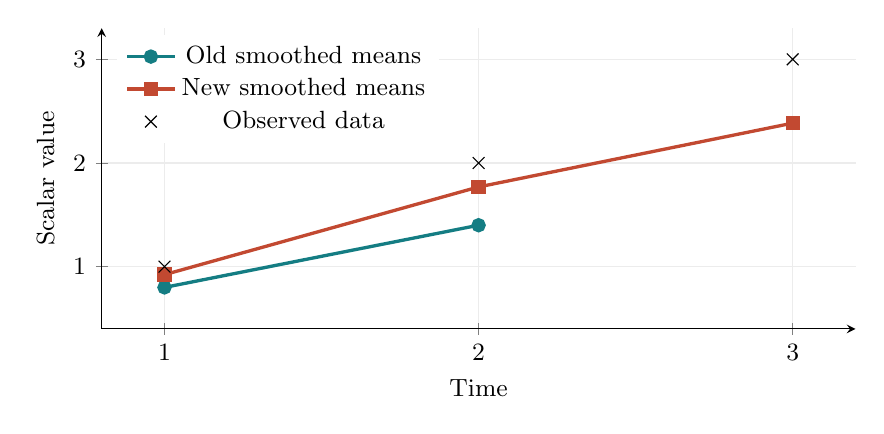
\begin{tikzpicture}
\begin{axis}[width=.92\linewidth,height=5.4cm,xmin=.8,xmax=3.2,ymin=.4,ymax=3.3,
xtick={1,2,3},xlabel={Time},ylabel={Scalar value},axis lines=left,
grid=major,grid style={gray!15},legend style={font=\small,draw=none,at={(.02,.98)},anchor=north west},
tick label style={font=\small},label style={font=\small}]
\addplot[teal,line width=1.2pt,mark=*] coordinates {(1,.8)(2,1.4)};
\addlegendentry{Old smoothed means}
\addplot[red,line width=1.2pt,mark=square*] coordinates {(1,.923076923)(2,1.769230769)(3,2.384615385)};
\addlegendentry{New smoothed means}
\addplot[black,only marks,mark=x,mark size=3pt] coordinates {(1,1)(2,2)(3,3)};
\addlegendentry{Observed data}
\end{axis}\end{tikzpicture}
\end{center}
The new observation raises both historical means. We did not reuse $y_1,y_2$ as fresh
likelihood factors; their information and historical dependence were already in $(m,C)$.

\clearpage
\section*{6. Updating an unknown parameter as well}
To make parameter learning explicit while keeping all calculations exact, now let the
state-innovation variance be unknown with a two-point prior:
\[
\Pr(q=1)=\Pr(q=4)=\tfrac12.
\]
Keep $x_1\sim\Normal(0,1)$ independent of $q$, $R=1$, and the same three observations.
For each value of $q$, the conditional state model is Gaussian. The joint posterior is
represented by a weight $w_T(q)$ and a full-path Gaussian with mean $m_q$ and covariance $C_q$.

\textbf{Exact sequential algorithm, when the new observation arrives:}
\begin{enumerate}
\item For each $q\in\{1,4\}$, apply the prediction and full-path update from page 2 to
obtain $(m_q^+,C_q^+)$. This smooths every state conditional on that value of $q$.
\item Calculate the new predictive likelihood using the old posterior:
\[
\ell_q=p(y_{T+1}\mid y_{1:T},q)
=\Normal\bigl(y_{T+1};(m_q)_T,(C_q)_{TT}+q+R\bigr).
\]
\item Update the parameter weights using only that new likelihood:
\[
\boxed{w_{T+1}(q)=\frac{w_T(q)\ell_q}{\sum_{q'}w_T(q')\ell_{q'}}.}
\]
\item Retain both the updated weights and the updated conditional path distributions.
The smoothed state posterior is their Gaussian mixture, not generally a single Gaussian:
\[
p(X_{T+1}\mid y_{1:T+1})
=\sum_{q\in\{1,4\}}w_{T+1}(q)\Normal(X_{T+1};m_q^+,C_q^+).
\]
\end{enumerate}

\begin{center}\small
\begin{tabular}{lrrrr}\toprule
& Original prior & After $y_1,y_2$ & New likelihood $\ell_q$ & After $y_1,y_2,y_3$\\\midrule
$q=1$ & .500000 & .537125 & .151223 & .549440\\
$q=4$ & .500000 & .462875 & .143900 & .450560\\\bottomrule
\end{tabular}
\end{center}
Consequently, $\E[q\mid y_{1:2}]=2.388625$ changes to
$\E[q\mid y_{1:3}]=2.351679$. The conditional smoothed means after the update are
\[
m_1^+=\frac1{13}(12,23,31)',\qquad
m_4^+=\frac1{32}(21,61,89)'.
\]
Combining these with the \emph{new} weights gives
\[
\E[X_3\mid y_{1:3}]=(0.802855,\;1.830966,\;2.563323)'.
\]
Thus the new observation updates the parameter distribution \emph{and} the whole state path.
For a joint draw, first draw $q$ from its updated probabilities, then draw the entire path
from its corresponding Gaussian. This preserves parameter--state dependence.

\textbf{Why batch still agrees.} For each $q$,
$w_T(q)\propto p(q)p(y_{1:T}\mid q)$, so multiplying by $\ell_q$ gives
$w_{T+1}(q)\propto p(q)p(y_{1:T+1}\mid q)$.
The conditional Gaussian paths also agree with batch conditioning, so the full joint
posterior of $(q,X_{T+1})$ agrees, not just its means.

\textbf{What this means for DSC.} The same identity applies to its joint parameter and
state posterior. Preserve parameter--state and cross-time dependence, keep the original
prior and calibration fixed, and introduce the new transition and observation once.
For a nonlinear model, a practical sequential sampler approximates this distribution;
finite Monte Carlo results need not match a fresh batch run exactly. Holding saved parameter
means fixed and smoothing states is not the same as updating the joint posterior.

{\footnotesize\textbf{Verification.} All examples were checked independently by sequential
conditioning and batch matrix calculations, including the parameter weights.
Reproduce with \texttt{python3 scripts/verify\_sequential\_bayes\_scalar.py}.
\textbf{Further reading.} S\"arkk\"a and Svensson (2023),
\emph{Bayesian Filtering and Smoothing}, 2nd ed.,
\href{https://www.cambridge.org/core/books/abs/bayesian-filtering-and-smoothing/batch-and-recursive-bayesian-estimation/720DF1C5D896F74B03921B0FB4E020B1}{Chapter 3: Batch and Recursive Bayesian Estimation}.
}
\end{document}
